\documentclass[12pt, a4paper]{article}

\usepackage{CJKutf8}
\usepackage{graphicx}

\title{Timelog}
\author{105820009 汪秉沄\\
108598074 顏翊純\\
105820014 張雅雯\\
105820026 張景博\\
108598047 胡喻翔}
\date{\today}

\begin{document}
\begin{CJK*}{UTF8}{bkai}
\pagenumbering{gobble}
\maketitle
\newpage

\tableofcontents
\newpage

\pagenumbering{arabic}

\section{Requirement Document}
  \subsection{Change History}
  3/23 Ten use cases added,\\
    \indent use case diagram added,\\
    \indent context diagram added,\\
    \indent Non-functional Requirements and Constraints,\\
  3/22 Four use cases added\\
  3/10 Problem Statement added\\

  \subsection{Problem Statement}
  \paragraph{}
  敏捷開發逐漸成為主流,其中以Scrum最為著名,然而現在卻沒有能夠讓
使用者完全倚賴的 Scrum 管理軟體。軟體系統實驗室現有的 ezScrum 系統並不 適合讓剛接觸 Scrum 的人上手,甚至對 Scrum 流程不熟悉的人容易對 Scrum 產 生錯誤的理解。此外,Scrum 的附屬行為仍然需要搭配實際的工具與活動,這 造成了資源的浪費、團隊在某些特定情況下 Scrum 活動難以順利進行。當今業 界中有名的 Jira 軟體,試圖一次將太多資訊夾雜在有限的介面中,也並未符合 Scrum 中定義的各種資訊,不僅在使用上混亂,而且對於團體的新人、甚至是 Scrum初學者,需要一次面對太大量的資訊與過於複雜的介面。

因此我們希望開發一套 Scrum 管理系統,提供一個流程動態視覺化的介 面,幫助團隊不只記錄,更可以將他們的開發流程更好的視覺化,讓新手可以 快速地理解 Scrum 的各個流程活動;老手也能輕易掌握 Scrum 運行的狀況。此 外,這個系統也需要提供數個虛擬化的 Scrum 常用工具,並提供使用者客製化 的彈性空間,使其更貼近各個團隊的使用狀況。而前述的所有軟體都缺乏一個 完整的 Dash Board 介面,讓使用者始終無法真正脫離實際的 Task Board、 Burndown Chart 等工具;因此這套系統需要提供這樣的介面,讓 Scrum 的流程 管理可以真正的虛擬化。

  \subsection{System Context Diagram}
    \begin{figure}[h!]
      \centering
      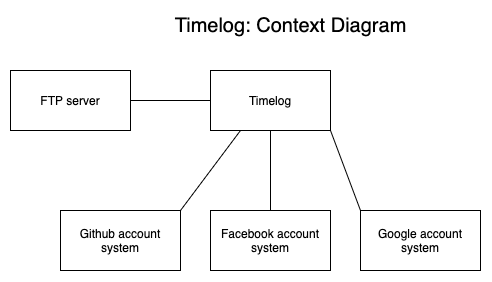
\includegraphics[width=\linewidth]{img/Context_Diagram.png}
    \end{figure}

  \subsection{Summary of System Feature}
    \begin{itemize}
      \item Team management
      \item Log record
      \item Serveral third part login methods
      \item Upload report to an FTP server.
      \item User's goal to help to improve user's time allocation.
    \end{itemize}

  \subsection{Use Case Diagram}
    \begin{figure}[h!]
      \centering
      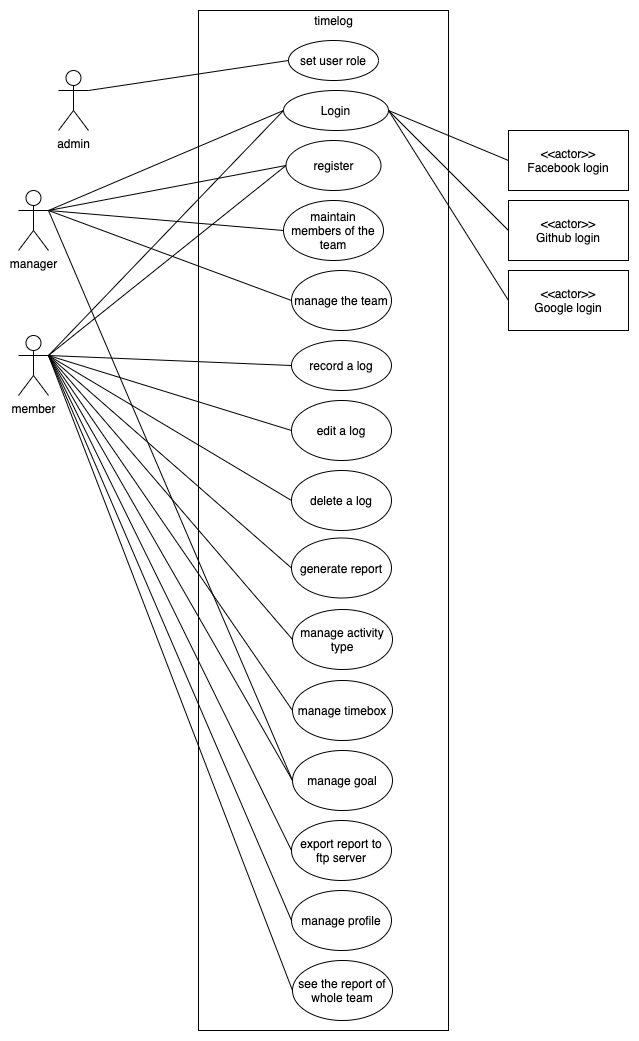
\includegraphics[width=\linewidth]{img/usecase_diagram/Usecase_diagram.png}
    \end{figure}

  \subsection{Use Cases}
    \begin{enumerate}
      \item Manage user account
        \begin{itemize}
          \item Scope: Account Management System
          \item Level: subfunction
          \item Primary Actor: User
          \item Stakeholders and Interests:
            \begin{itemize}
              \item {\bf Member}: A teammeber wants to login to Timelog to record and maintain their own logs.
              \item {\bf Manager}: A manager wants to be able to maintain the members of team, and see teammebers' timelog report.
              \item {\bf Organization}: With several teams in an organization, we a group to association with user account to maintain the members easily.
            \end{itemize}
          \item Preconditions: None.
          \item Success Guarantee:
            \begin{itemize}
              \item User register account
              \item User login to system.
              \item Logs are distinguished by users identity.
              \item Manager maintain users of the team.
              \item Users see the logs reports of other team members of the same team.
            \end{itemize}
          \item Main Success Scenario: User login to timelog
            \begin{enumerate}
              \item User enter Timelog page.
              \item Direct user to login page.
              \item User select a login method to login to system.
                \begin{itemize}
                  \item {\bf FB login}
                    \begin{enumerate}
                      \item System redirect user to FB login page.
                      \item User enter Facebook account info to login.
                    \end{enumerate}
                  \item {\bf Google login}
                    \begin{enumerate}
                      \item System redirect user to Google login page.
                      \item User enter Google account info to login.
                    \end{enumerate}
                  \item {\bf Github login}
                    \begin{enumerate}
                      \item System redirect user to Github login service.
                      \item User enter Github account info to login.
                    \end{enumerate}
                \end{itemize}
              \item System redirects the user back to Timelog page.
              \item User logined to timelog.
            \end{enumerate}
          \item Extensions:
            \begin{enumerate}
              \item User register an account
              \begin{enumerate}
                \item User enters to Timelog page.
                \item System redirects user to login page.
                \item User selects to register an account.
                \item User inputs the basic information.
                \item User creates an account
              \end{enumerate}
              \item User autologin
                \begin{enumerate}
                  \item User enter to Timelog page.
                  \item If user login with same device before.
                  \item The System auto login for user.
                  \item User enter the system.
                \end{enumerate}
              \item If user give the wrong login information.
                \begin{enumerate}
                  \item User enter to Timelog page.
                  \item User entered incorrect account or password
                  \item System reject login.
                \end{enumerate}
              \item Manager manage team members of a team.
                \begin{enumerate}
                  \item Manager enter team manage page.
                  \item Manager do manage operations to manage the members in the team.
                    \begin{itemize}
                      \item Add user to the team.
                      \item Remove a member from the team.
                      \item Set role of the team to a member.
                    \end{itemize}
                  \item The team members' team information updated.
                \end{enumerate}
            \end{enumerate}
          \item Special Requirements:
            \begin{enumerate}
              \item Provide an identity to distinguish logs.
              \item User should be able to connect their account with several third part oauth services, such as FB, Google, Github.
              \item Record user's login status.
            \end{enumerate}
          \item Technology and Data Variations List:
            \begin{enumerate}
              \item User can login through thee kinds of third part login, including Facebook, Google, and Github.
              \item A user may have role in a team, manager or normal member, with different authority to team management
            \end{enumerate}
          \item Frequency of Occurrence: Every time an user wants to use Timelog.
          \item Miscellaneous:
            \begin{itemize}
              \item Open Issues:
                \begin{itemize}
                  \item How long should user token expired?
                  \item What roles should we have for members in a team?
                \end{itemize}
            \end{itemize}
        \end{itemize}
      \item User manage logs
        \begin{itemize}
          \item Scope: Timelog system
          \item Level: User-goal
          \item Primary Actor: user
          \item Stakeholders and Interests:
            \begin{itemize}
              \item {\bf User}: User wants to record his/her life activities to monitor him/her self time usage to improve his/her time management.
            \end{itemize}
          \item Preconditions:
            \begin{itemize}
              \item User logined
              \item User set activity types.
            \end{itemize}
          \item Success Guarantee:
            \begin{itemize}
              \item User record a log to the system.
              \item User edit a log in the system.
              \item User delete a log in the system.
            \end{itemize}
          \item Main Success Scenario: User record a log.
            \begin{enumerate}
              \item User logined to Timelog.
              \item User send "Record Log" command
              \item User input informations needed for a log.
                \begin{itemize}
                  \item Title
                  \item Time period
                  \item Activity Type
                  \item Description
                \end{itemize}
            \end{enumerate}
          \item Extensions:
            \begin{enumerate}
              \item User edit log.
                \begin{enumerate}
                  \item User select an incorrect log.
                  \item User inputs the new information of log.
                  \item User update the selected log.
                \end{enumerate}
              \item User delete a log
                \begin{enumerate}
                  \item User select a log.
                  \item User delete the selected log.
                \end{enumerate}
            \end{enumerate}
          \item Special Requirements: None
          \item Technology and Data Variations List:
            \begin{itemize}
              \item Activity types are several types defined by the user.
            \end{itemize}
          \item Frequency of Occurrence: an hour to a day.
          \item Miscellaneous: None
        \end{itemize}
      \item System generates report
        \begin{itemize}
          \item Scope: Timelog System
          \item Level: User-goal
          \item Primary Actor: Timelog System
          \item Stakeholders and Interests:
            \begin{itemize}
              \item {\bf User}: User see the report of selected period or timebox, so he/she can know how did his/her time have been spent.
              \item {\bf Manager}: Manager wants to see the the time allocation of his/her team members, to analysis the working quality of the team.
            \end{itemize}
          \item Preconditions:
            \begin{itemize}
              \item Log added.
              \item Activity types added.
              \item Timebox created.
              \item Goal of activities set.
            \end{itemize}
          \item Success Guarantee:
            \begin{itemize}
              \item Pie chart and table report generated.
              \item the data of report is in the range of selected period/Timebox
              \item Goal complete rate report generated.
            \end{itemize}
          \item Main Success Scenario:
            \begin{enumerate}
              \item User's operations satisfied all preconditions.
              \item System generates the report according to Timebox, activity types, goal, and logs.
              \item Reports showed on web page.
            \end{enumerate}
          \item Extensions:
            \begin{enumerate}
              \item Report without goal.
                \begin{enumerate}
                  \item If user didn't set goal for current Timebox.
                  \item System generates the report accoring to Timebox, activity types, and logs(wihtout goal).
                  \item Reports showed on web page (wihtout goal).
                \end{enumerate}
            \end{enumerate}
          \item Special Requirements:
            \begin{enumerate}
              \item User can specify a period, instead of Timebox to generate report.
            \end{enumerate}
          \item Technology and Data Variations List:
            \begin{itemize}
              \item Duration of report could be Timebox, or user selected period.
              \item Goal report showed only if user sets at least one goal.
            \end{itemize}
          \item Frequency of Occurrence: Every time user add a new log.
          \item Miscellaneous:
            \begin{itemize}
              \item Should we provide more than one chart rather than pie chart only?
              \item What information to show on report?
            \end{itemize}
        \end{itemize}
      \item User manage Activity Type
        \begin{itemize}
          \item Scope: Timelog System
          \item Level: User-goal
          \item Primary Actor: user
          \item Stakeholders and Interests:
            \begin{itemize}
              \item {\bf User}: User needs activity type
            \end{itemize}
          \item Preconditions: User logined to Timelog.
          \item Success Guarantee:
            \begin{itemize}
              \item User add an Activity Type
              \item User edit an Activity Type
              \item User delete an Activity Type
            \end{itemize}
          \item Main Success Scenario: User add an activity type.
            \begin{enumerate}
              \item User logins to Timelog
              \item User enters Activity Type management page
              \item User inputs information for new Activity Type.
              \item User triggers "add" command.
              \item The new Activity Type added to user's account.
            \end{enumerate}
          \item Extensions:
            \begin{itemize}
              \item At any time, if user leaves setting page, the add operation is canceled.
              \item User edits an Activity Type.
                \begin{enumerate}
                  \item User logins to timelog.
                  \item User enters Activity Type management page.
                  \item User selects an existed Activity Type.
                  \item User gives an edit command.
                  \item User updates new informations for the type.
                  \item User gives an update command.
                  \item The selected Activity Type is updated.
                \end{enumerate}
              \item User deletes an Activity Type.
                \begin{enumerate}
                  \item User logins to timelog.
                  \item User enters Activity Type management page.
                  \item User selects an existed Activity Type.
                  \item User gives an delete command.
                  \item The selected Activity Type is deleted.
                \end{enumerate}
            \end{itemize}
          \item Special Requirements:
            \begin{itemize}
              \item The users should be able to open Activity Type management while adding a new log, to simplify the add log process.
            \end{itemize}
          \item Technology and Data Variations List:
            \begin{itemize}
              \item Activity Type management can either be a page, user selects the management subpage, or a popup window, user triggers while adding a log.
            \end{itemize}
          \item Frequency of Occurrence: Mostly few month or even years, according to the life event of the user.
          \item Miscellaneous:
            \begin{itemize}
              \item What information should we have except for type name?
              \item Is there a limit for number of activities?
            \end{itemize}
        \end{itemize}
      \item Export report to FTP server
        \begin{itemize}
          \item Scope: Timelog System
          \item Level: subfunction
          \item Primary Actor: User
          \item Stakeholders and Interests:
            \begin{itemize}
              \item {\bf User}: User export and upload the report to the shared FTP server, so other members of the organization can see the log.
              \item {\bf Manager}: An organization manager can see the reports of members on a manual service based on an FTP server.
              \item {\bf Organization}: We can have a self hosted FTP server to record all the reports of organization members.
            \end{itemize}
          \item Preconditions:
            \begin{itemize}
              \item User set acitivty types
              \item User add logs
              \item User set Timebox
              \item User set goal(Not required)
            \end{itemize}
          \item Success Guarantee: The report is generated an uploaded to FTP server.
          \item Main Success Scenario: Report exported and uploaded to FTP server.
            \begin{itemize}
              \item User logins to Timelog
              \item User selects an Timebox
              \item User gives export command
              \item User sets FTP server authorization info.
              \item The system generates an report and uploads to the specified FTP server.
            \end{itemize}
          \item Extensions: None
          \item Special Requirements:
            \begin{itemize}
              \item If user exported a report before, the system should auto fill the FTP info for the user.
            \end{itemize}
          \item Technology and Data Variations List:
            \begin{itemize}
              \item Upload can through either FTP or FTPs protocol.
            \end{itemize}
          \item Frequency of Occurrence: Weekly or monthly, according to the organization's policy.
          \item Miscellaneous: None
        \end{itemize}
      \item User manage profile
        \begin{itemize}
          \item Scope: Account Management service
          \item Level: subfunction
          \item Primary Actor: User
          \item Stakeholders and Interests:
            \begin{itemize}
              \item {\bf User}: A user wants to add/update personal profile whenever personal information changed.
              \item {\bf Other members}: A member might need to know some basic information of others to complete some task, for example, contact information such as phone or email.
            \end{itemize}
          \item Preconditions:
            \begin{itemize}
              \item User registered an account.
            \end{itemize}
          \item Success Guarantee:
            \begin{itemize}
              \item The profile updated
            \end{itemize}
          \item Main Success Scenario:
            \begin{enumerate}
              \item User enters profile manage page.
              \item User selects an item to update.
              \item User fills in the information.
              \item User updates the information.
            \end{enumerate}
          \item Extensions:
            \begin{itemize}
              \item The user enter another user's profile page, andsee the shared profile of the another user.
            \end{itemize}
          \item Special Requirements: None
          \item Technology and Data Variations List: None
          \item Frequency of Occurrence: Rare, only if personal information changed.
          \item Miscellaneous: None
        \end{itemize}
      \item Maintain Timebox
        \begin{itemize}
          \item Scope: Timelog service
          \item Level: User-goal
          \item Primary Actor: User
          \item Stakeholders and Interests:
            \begin{itemize}
              \item {\bf User}: A user needs a Timebox to get the reports in the period that he/she is interested.
              \item {\bf Manager}: A manager wants to check the team members' log reports in a constant pace iteratively.
            \end{itemize}
          \item Preconditions:
            \begin{itemize}
              \item User login to Timelog.
            \end{itemize}
          \item Success Guarantee:
            \begin{itemize}
              \item User sets up an Timebox.
              \item System generates report according to the Timebox.
            \end{itemize}
          \item Main Success Scenario: A Timebox defined
            \begin{enumerate}
              \item User enters Timelog system.
              \item User gives "Create Timebox" command.
              \item User inputs name, description, and period of iteration.
              \item User gives Create command.
              \item Timebox created.
            \end{enumerate}
          \item Extensions:
            \begin{itemize}
              \item User changes current Timebox, the system should generates report according to the new selected Timebox.
            \end{itemize}
          \item Special Requirements:
            \begin{itemize}
              \item The start date of Timebox should not overlap the end date.
            \end{itemize}
          \item Technology and Data Variations List:
            \begin{itemize}
              \item Despite specifying a static long term Timebox, user can simply select a period of time as temporary Timebox.
            \end{itemize}
          \item Frequency of Occurrence: Weekly, two weeks a time, monthly, etc. According to user's habbit or organization's policy.
          \item Miscellaneous: None
        \end{itemize}
      \item Maintain goal of timebox
        \begin{itemize}
          \item Scope: Timelog System
          \item Level: user-goal
          \item Primary Actor: User
          \item Stakeholders and Interests:
            \begin{itemize}
              \item {\bf User}: A user sets goal of a Timebox for each activity to visualize user's time allocation quality, and help user to improve their time allocation eventually.
            \end{itemize}
          \item Preconditions:
            \begin{itemize}
              \item User defined activity types.
              \item User set a Timebox
            \end{itemize}
          \item Success Guarantee:
            \begin{itemize}
              \item User set goals for several activities.
              \item Goal achievement of each activity be shown on the report.
            \end{itemize}
          \item Main Success Scenario:
            \begin{enumerate}
              \item User selects a Timebox
              \item User gives "Set goals" command
              \item User define the goal hour of each activities.
              \item After that, the system will add goal achievement to the report of the selected Timebox.
            \end{enumerate}
          \item Extensions: None
          \item Special Requirements: None
          \item Technology and Data Variations List:
            \begin{itemize}
              \item A goal of an activity can either be a positive value, the hour of goal is set, or 0, no goal for the activity; a negitive value is not acceptable.
            \end{itemize}
          \item Frequency of Occurrence: Every time a new Timebox created.
          \item Miscellaneous:
            \begin{itemize}
              \item Despite hour goal, is there any other good measurement for goal to visualize user's time allocation quality?
            \end{itemize}
        \end{itemize}
      \item Team member see the report of whole team \& other members.
        \begin{itemize}
          \item Scope: Timelog service
          \item Level: subfunction
          \item Primary Actor: Member
          \item Stakeholders and Interests:
            \begin{itemize}
              \item {\bf Member}: Team members want to see the report of whole team and other members to know how team's working status is.
              \item {\bf Manager}: A Manager wants to see the report of whole team and other members to be a reference to analysis team's working quality and passion.
            \end{itemize}
          \item Preconditions:
            \begin{itemize}
              \item Members added to the team.
              \item The manager set Timebox and goal for the team.
            \end{itemize}

          \item Success Guarantee:
          \item Main Success Scenario:
          \item Extensions:
          \item Special Requirements:
          \item Technology and Data Variations List:
          \item Frequency of Occurrence:
          \item Miscellaneous:
        \end{itemize}
      \item Manage the team.
        \begin{itemize}
          \item Scope: Account management system
          \item Level: User-goal
          \item Primary Actor: Manager
          \item Stakeholders and Interests:
            \begin{itemize}
              \item {\bf Manager}: A manager wants to create a team, and maintain the members due to the team status in real life.
            \end{itemize}
          \item Preconditions:
            \begin{itemize}
              \item user account created
            \end{itemize}
          \item Success Guarantee:
            \begin{itemize}
              \item Manager created a team.
              \item Manager maintain the members in the team.
            \end{itemize}
          \item Main Success Scenario:
            \begin{enumerate}
              \item Manager enters team mangement system.
              \item Manager creates a team.
              \item Manager adds users to the team.
            \end{enumerate}
          \item Extensions:
            \begin{itemize}
              \item If a manager tries to create an existing team, the operation should be rejected.
              \item Member leave the team
                \begin{enumerate}
                  \item Manager enters the team management system of the team.
                  \item Manager select the leaved member.
                  \item Manager remove the member from the team.
                \end{enumerate}
              \item New member join the team
                 \begin{enumerate}
                  \item Manager enters the team management system of the team.
                  \item Manager select the leaved member.
                  \item Manager add the new member to the team.
                 \end{enumerate}
              \item Manager creates subteams.
                \begin{enumerate}
                  \item Manager enters the team management system of the team.
                  \item Manager creates a sub team of the team.
                \end{enumerate}
            \end{itemize}
          \item Special Requirements:
            \begin{itemize}
              \item Team name should not be duplicated
            \end{itemize}
          \item Technology and Data Variations List:
          \item Frequency of Occurrence: Once there's personnel changes in the team.
          \item Miscellaneous:
        \end{itemize}
      \item Admin set role to users.
        \begin{itemize}
          \item Scope: Account Mangement System
          \item Level: subfunction
          \item Primary Actor: Admin
          \item Stakeholders and Interests:
            \begin{itemize}
              \item {\bf Admin}: an administrator have to manage users' roles.
            \end{itemize}
          \item Preconditions: None
          \item Success Guarantee:
            \item User roles updated.
          \item Main Success Scenario:
            \begin{enumerate}
              \item Admin enter admin area.
              \item Admin select user.
              \item Admin set new roles of user.
            \end{enumerate}
          \item Extensions: None
          \item Special Requirements: None
          \item Technology and Data Variations List: None
          \item Frequency of Occurrence: Very rare.
          \item Miscellaneous: None
        \end{itemize}
      \item Manager set timebox and goal for team.
        \begin{itemize}
          \item Scope: Timelog System
          \item Level: User-goal
          \item Primary Actor: Manager
          \item Stakeholders and Interests:
            \begin{itemize}
              \item {\bf Manager}: A manager wants to set the timebox and goal for the team to help to analysis team working quality.
            \end{itemize}
          \item Preconditions:
            \begin{itemize}
              \item A team created
            \end{itemize}
          \item Success Guarantee:
            \begin{itemize}
              \item Timebox created.
              \item Goal of timebox set.
            \end{itemize}
          \item Main Success Scenario: Create a timebox and set goal
            \item Manager enters team management page
            \item Manager set a time period as Timebox
            \item Manager user set goal of activities of the Timebox
            \item System generates a report of the team according to the team timebox and team goal
          \item Extensions:
            \begin{itemize}
              \item If the period is not correct, system will rejected.
              \item If the goal is not correct, system will rejected.
            \end{itemize}
          \item Special Requirements: None
          \item Technology and Data Variations List: None
          \item Frequency of Occurrence: None
          \item Miscellaneous: None
        \end{itemize}
      \item User set background color.
        \begin{itemize}
          \item Scope: Timelog System
          \item Level: User-goal
          \item Primary Actor: User
          \item Stakeholders and Interests:
            \begin{itemize}
              \item {\bf User}: A user wants to set the background color.
            \end{itemize}
          \item Preconditions: None
          \item Success Guarantee:
            \begin{itemize}
              \item A background color is set
            \end{itemize}
          \item Main Success Scenario:
            \begin{itemize}
              \item If user does not save the changes, system will ignore the changes.
            \end{itemize}
          \item Extensions:
            \begin{itemize}
              \item If user does not save the changes, system will ignore the changes.
            \end{itemize}
          \item Special Requirements: None
          \item Technology and Data Variations List: None
          \item Frequency of Occurrence: None
          \item Miscellaneous: None
        \end{itemize}
    \end{enumerate}
  \subsection{Non-functional Requirements and Constraints}
    \begin{itemize}
      \item Page switch time should less than 3 seconds.
      \item Backend response time should less than 1 seconds.
      \item report generate time should less than 1 seconds.
      \item All user identity transmited between server and client should be access token.
    \end{itemize}
    \begin{itemize}
      \item Browser that support ex5 plus.
    \end{itemize}
  \subsection{Glossary}

  \subsection{Software Environments}
    \begin{itemize}
      \item Java JDK 1.8
      \item React.js
    \end{itemize}

\section{Measurement}


\end{CJK*}
\end{document}
